% Options for packages loaded elsewhere
\PassOptionsToPackage{unicode}{hyperref}
\PassOptionsToPackage{hyphens}{url}
%
\documentclass[
]{article}
\usepackage{amsmath,amssymb}
\usepackage{lmodern}
\usepackage{iftex}
\ifPDFTeX
  \usepackage[T1]{fontenc}
  \usepackage[utf8]{inputenc}
  \usepackage{textcomp} % provide euro and other symbols
\else % if luatex or xetex
  \usepackage{unicode-math}
  \defaultfontfeatures{Scale=MatchLowercase}
  \defaultfontfeatures[\rmfamily]{Ligatures=TeX,Scale=1}
\fi
% Use upquote if available, for straight quotes in verbatim environments
\IfFileExists{upquote.sty}{\usepackage{upquote}}{}
\IfFileExists{microtype.sty}{% use microtype if available
  \usepackage[]{microtype}
  \UseMicrotypeSet[protrusion]{basicmath} % disable protrusion for tt fonts
}{}
\makeatletter
\@ifundefined{KOMAClassName}{% if non-KOMA class
  \IfFileExists{parskip.sty}{%
    \usepackage{parskip}
  }{% else
    \setlength{\parindent}{0pt}
    \setlength{\parskip}{6pt plus 2pt minus 1pt}}
}{% if KOMA class
  \KOMAoptions{parskip=half}}
\makeatother
\usepackage{xcolor}
\usepackage[margin=1in]{geometry}
\usepackage{color}
\usepackage{fancyvrb}
\newcommand{\VerbBar}{|}
\newcommand{\VERB}{\Verb[commandchars=\\\{\}]}
\DefineVerbatimEnvironment{Highlighting}{Verbatim}{commandchars=\\\{\}}
% Add ',fontsize=\small' for more characters per line
\usepackage{framed}
\definecolor{shadecolor}{RGB}{248,248,248}
\newenvironment{Shaded}{\begin{snugshade}}{\end{snugshade}}
\newcommand{\AlertTok}[1]{\textcolor[rgb]{0.94,0.16,0.16}{#1}}
\newcommand{\AnnotationTok}[1]{\textcolor[rgb]{0.56,0.35,0.01}{\textbf{\textit{#1}}}}
\newcommand{\AttributeTok}[1]{\textcolor[rgb]{0.77,0.63,0.00}{#1}}
\newcommand{\BaseNTok}[1]{\textcolor[rgb]{0.00,0.00,0.81}{#1}}
\newcommand{\BuiltInTok}[1]{#1}
\newcommand{\CharTok}[1]{\textcolor[rgb]{0.31,0.60,0.02}{#1}}
\newcommand{\CommentTok}[1]{\textcolor[rgb]{0.56,0.35,0.01}{\textit{#1}}}
\newcommand{\CommentVarTok}[1]{\textcolor[rgb]{0.56,0.35,0.01}{\textbf{\textit{#1}}}}
\newcommand{\ConstantTok}[1]{\textcolor[rgb]{0.00,0.00,0.00}{#1}}
\newcommand{\ControlFlowTok}[1]{\textcolor[rgb]{0.13,0.29,0.53}{\textbf{#1}}}
\newcommand{\DataTypeTok}[1]{\textcolor[rgb]{0.13,0.29,0.53}{#1}}
\newcommand{\DecValTok}[1]{\textcolor[rgb]{0.00,0.00,0.81}{#1}}
\newcommand{\DocumentationTok}[1]{\textcolor[rgb]{0.56,0.35,0.01}{\textbf{\textit{#1}}}}
\newcommand{\ErrorTok}[1]{\textcolor[rgb]{0.64,0.00,0.00}{\textbf{#1}}}
\newcommand{\ExtensionTok}[1]{#1}
\newcommand{\FloatTok}[1]{\textcolor[rgb]{0.00,0.00,0.81}{#1}}
\newcommand{\FunctionTok}[1]{\textcolor[rgb]{0.00,0.00,0.00}{#1}}
\newcommand{\ImportTok}[1]{#1}
\newcommand{\InformationTok}[1]{\textcolor[rgb]{0.56,0.35,0.01}{\textbf{\textit{#1}}}}
\newcommand{\KeywordTok}[1]{\textcolor[rgb]{0.13,0.29,0.53}{\textbf{#1}}}
\newcommand{\NormalTok}[1]{#1}
\newcommand{\OperatorTok}[1]{\textcolor[rgb]{0.81,0.36,0.00}{\textbf{#1}}}
\newcommand{\OtherTok}[1]{\textcolor[rgb]{0.56,0.35,0.01}{#1}}
\newcommand{\PreprocessorTok}[1]{\textcolor[rgb]{0.56,0.35,0.01}{\textit{#1}}}
\newcommand{\RegionMarkerTok}[1]{#1}
\newcommand{\SpecialCharTok}[1]{\textcolor[rgb]{0.00,0.00,0.00}{#1}}
\newcommand{\SpecialStringTok}[1]{\textcolor[rgb]{0.31,0.60,0.02}{#1}}
\newcommand{\StringTok}[1]{\textcolor[rgb]{0.31,0.60,0.02}{#1}}
\newcommand{\VariableTok}[1]{\textcolor[rgb]{0.00,0.00,0.00}{#1}}
\newcommand{\VerbatimStringTok}[1]{\textcolor[rgb]{0.31,0.60,0.02}{#1}}
\newcommand{\WarningTok}[1]{\textcolor[rgb]{0.56,0.35,0.01}{\textbf{\textit{#1}}}}
\usepackage{graphicx}
\makeatletter
\def\maxwidth{\ifdim\Gin@nat@width>\linewidth\linewidth\else\Gin@nat@width\fi}
\def\maxheight{\ifdim\Gin@nat@height>\textheight\textheight\else\Gin@nat@height\fi}
\makeatother
% Scale images if necessary, so that they will not overflow the page
% margins by default, and it is still possible to overwrite the defaults
% using explicit options in \includegraphics[width, height, ...]{}
\setkeys{Gin}{width=\maxwidth,height=\maxheight,keepaspectratio}
% Set default figure placement to htbp
\makeatletter
\def\fps@figure{htbp}
\makeatother
\setlength{\emergencystretch}{3em} % prevent overfull lines
\providecommand{\tightlist}{%
  \setlength{\itemsep}{0pt}\setlength{\parskip}{0pt}}
\setcounter{secnumdepth}{-\maxdimen} % remove section numbering
\ifLuaTeX
  \usepackage{selnolig}  % disable illegal ligatures
\fi
\IfFileExists{bookmark.sty}{\usepackage{bookmark}}{\usepackage{hyperref}}
\IfFileExists{xurl.sty}{\usepackage{xurl}}{} % add URL line breaks if available
\urlstyle{same} % disable monospaced font for URLs
\hypersetup{
  hidelinks,
  pdfcreator={LaTeX via pandoc}}

\author{}
\date{\vspace{-2.5em}}

\begin{document}

\textbf{Question 1}

\begin{Shaded}
\begin{Highlighting}[]
\FunctionTok{library}\NormalTok{(resampledata)}
\end{Highlighting}
\end{Shaded}

\begin{verbatim}
## 
## Attaching package: 'resampledata'
\end{verbatim}

\begin{verbatim}
## The following object is masked from 'package:datasets':
## 
##     Titanic
\end{verbatim}

\begin{Shaded}
\begin{Highlighting}[]
\FunctionTok{library}\NormalTok{(mosaic)}
\end{Highlighting}
\end{Shaded}

\begin{verbatim}
## Registered S3 method overwritten by 'mosaic':
##   method                           from   
##   fortify.SpatialPolygonsDataFrame ggplot2
\end{verbatim}

\begin{verbatim}
## 
## The 'mosaic' package masks several functions from core packages in order to add 
## additional features.  The original behavior of these functions should not be affected by this.
\end{verbatim}

\begin{verbatim}
## 
## Attaching package: 'mosaic'
\end{verbatim}

\begin{verbatim}
## The following objects are masked from 'package:dplyr':
## 
##     count, do, tally
\end{verbatim}

\begin{verbatim}
## The following object is masked from 'package:Matrix':
## 
##     mean
\end{verbatim}

\begin{verbatim}
## The following object is masked from 'package:ggplot2':
## 
##     stat
\end{verbatim}

\begin{verbatim}
## The following objects are masked from 'package:stats':
## 
##     binom.test, cor, cor.test, cov, fivenum, IQR, median, prop.test,
##     quantile, sd, t.test, var
\end{verbatim}

\begin{verbatim}
## The following objects are masked from 'package:base':
## 
##     max, mean, min, prod, range, sample, sum
\end{verbatim}

\textbf{Q1. a.}

\begin{Shaded}
\begin{Highlighting}[]
\FunctionTok{tail}\NormalTok{(NCBirths2004, }\DecValTok{4}\NormalTok{)}
\end{Highlighting}
\end{Shaded}

\begin{verbatim}
##        ID MothersAge Tobacco Alcohol Gender Weight Gestation Smoker
## 1006 1006      20-24      No      No   Male   2835        39     No
## 1007 1007      15-19      No      No   Male   3260        38     No
## 1008 1008      20-24      No      No Female   2637        41     No
## 1009 1009      20-24      No      No Female   3005        39     No
\end{verbatim}

\begin{Shaded}
\begin{Highlighting}[]
\CommentTok{\#data.frame(table(NCBirths2004$Tobacco))}
\FunctionTok{data.frame}\NormalTok{(}\FunctionTok{table}\NormalTok{(NCBirths2004}\SpecialCharTok{$}\NormalTok{Smoker))}
\end{Highlighting}
\end{Shaded}

\begin{verbatim}
##   Var1 Freq
## 1   No  898
## 2  Yes  111
\end{verbatim}

\begin{Shaded}
\begin{Highlighting}[]
\CommentTok{\#dfno = NCBirths2004[NCBirths2004$Smoker == \textquotesingle{}No\textquotesingle{}, ]}
\CommentTok{\#dfyes = NCBirths2004[NCBirths2004$Smoker == \textquotesingle{}Yes\textquotesingle{}, ]}
\CommentTok{\#tail(dfyes, 4)}
\CommentTok{\#tail(dfno, 4)}
\FunctionTok{favstats}\NormalTok{(}\SpecialCharTok{\textasciitilde{}}\NormalTok{Weight}\SpecialCharTok{|}\NormalTok{Smoker, }\AttributeTok{data=}\NormalTok{NCBirths2004)}
\end{Highlighting}
\end{Shaded}

\begin{verbatim}
##   Smoker  min   Q1 median     Q3  max     mean       sd   n missing
## 1     No 2013 3147   3459 3771.0 5131 3471.912 478.5524 898       0
## 2    Yes 1928 2948   3204 3529.5 4649 3256.910 520.4788 111       0
\end{verbatim}

\begin{Shaded}
\begin{Highlighting}[]
\CommentTok{\#favstats(\textasciitilde{}Weight, data=dfyes)}
\NormalTok{nsims }\OtherTok{=} \DecValTok{1000} \CommentTok{\#the number of simulations}
\NormalTok{n.Yes }\OtherTok{=} \FunctionTok{favstats}\NormalTok{(}\SpecialCharTok{\textasciitilde{}}\NormalTok{Weight}\SpecialCharTok{|}\NormalTok{Smoker, }\AttributeTok{data=}\NormalTok{NCBirths2004)}\SpecialCharTok{$}\NormalTok{n[}\DecValTok{2}\NormalTok{] }
\NormalTok{n.No }\OtherTok{=} \FunctionTok{favstats}\NormalTok{(}\SpecialCharTok{\textasciitilde{}}\NormalTok{Weight}\SpecialCharTok{|}\NormalTok{Smoker, }\AttributeTok{data=}\NormalTok{NCBirths2004)}\SpecialCharTok{$}\NormalTok{n[}\DecValTok{1}\NormalTok{]}
\CommentTok{\#n.Yes}
\CommentTok{\#n.No}

\NormalTok{mean.NonSmoke }\OtherTok{=} \FunctionTok{numeric}\NormalTok{(nsims) }
\NormalTok{mean.YesSmoke }\OtherTok{=} \FunctionTok{numeric}\NormalTok{(nsims) }
\NormalTok{diffmeans }\OtherTok{=} \FunctionTok{numeric}\NormalTok{(nsims) }
\NormalTok{No }\OtherTok{=} \FunctionTok{filter}\NormalTok{(NCBirths2004, Smoker }\SpecialCharTok{==} \StringTok{\textquotesingle{}No\textquotesingle{}}\NormalTok{)  }
\NormalTok{Yes }\OtherTok{=} \FunctionTok{filter}\NormalTok{(NCBirths2004, Smoker }\SpecialCharTok{==} \StringTok{\textquotesingle{}Yes\textquotesingle{}}\NormalTok{)   }

\ControlFlowTok{for}\NormalTok{(i }\ControlFlowTok{in} \DecValTok{1}\SpecialCharTok{:}\NormalTok{nsims)}
\NormalTok{\{   mean.NonSmoke[i] }\OtherTok{=} \FunctionTok{mean}\NormalTok{(}\FunctionTok{sample}\NormalTok{(No}\SpecialCharTok{$}\NormalTok{Weight, n.No, }\AttributeTok{replace=}\ConstantTok{TRUE}\NormalTok{))  }
\NormalTok{    mean.YesSmoke[i] }\OtherTok{=} \FunctionTok{mean}\NormalTok{(}\FunctionTok{sample}\NormalTok{(Yes}\SpecialCharTok{$}\NormalTok{Weight, n.Yes, }\AttributeTok{replace=}\ConstantTok{TRUE}\NormalTok{)) }
\NormalTok{    diffmeans[i] }\OtherTok{=}\NormalTok{ mean.NonSmoke[i] }\SpecialCharTok{{-}}\NormalTok{ mean.YesSmoke[i]  }
\NormalTok{\}}
\NormalTok{boot.diffmeans }\OtherTok{=} \FunctionTok{data.frame}\NormalTok{(mean.NonSmoke, mean.YesSmoke, diffmeans)  }
\FunctionTok{head}\NormalTok{(boot.diffmeans, }\DecValTok{3}\NormalTok{)}
\end{Highlighting}
\end{Shaded}

\begin{verbatim}
##   mean.NonSmoke mean.YesSmoke diffmeans
## 1      3451.187      3245.423  205.7637
## 2      3480.430      3330.973  149.4569
## 3      3467.658      3319.991  147.6671
\end{verbatim}

\begin{Shaded}
\begin{Highlighting}[]
\FunctionTok{ggplot}\NormalTok{(}\AttributeTok{data=}\NormalTok{boot.diffmeans, }\FunctionTok{aes}\NormalTok{(}\AttributeTok{x =}\NormalTok{ diffmeans)) }\SpecialCharTok{+} \FunctionTok{geom\_histogram}\NormalTok{(}\AttributeTok{fill=}\StringTok{\textquotesingle{}blue\textquotesingle{}}\NormalTok{, }\AttributeTok{col=}\StringTok{\textquotesingle{}red\textquotesingle{}}\NormalTok{, }\AttributeTok{binwidth=}\DecValTok{25}\NormalTok{) }\SpecialCharTok{+} \FunctionTok{xlab}\NormalTok{(}\StringTok{"Difference Between Mean Weight(NonSmoke {-} Smoke)"}\NormalTok{) }\SpecialCharTok{+} \FunctionTok{ggtitle}\NormalTok{(}\StringTok{"Distribution of Mean\_\{NonSmoke\} {-} Mean\_\{Smoke\}"}\NormalTok{)}
\end{Highlighting}
\end{Shaded}

\includegraphics{A3_files/figure-latex/unnamed-chunk-1-1.pdf}

\textbf{Q1. b.}

\begin{Shaded}
\begin{Highlighting}[]
\FunctionTok{qdata}\NormalTok{(}\SpecialCharTok{\textasciitilde{}}\NormalTok{ diffmeans, }\FunctionTok{c}\NormalTok{(}\FloatTok{0.025}\NormalTok{, }\FloatTok{0.975}\NormalTok{), }\AttributeTok{data=}\NormalTok{boot.diffmeans) }
\end{Highlighting}
\end{Shaded}

\begin{verbatim}
##     2.5%    97.5% 
## 115.1336 320.3686
\end{verbatim}

From my result, the 95\% Bootstrap Confidence Interval is
\(111.8109 \leq \mu_{NonSmoke} - \mu_{Smoke} \leq 308.5742\)

\textbf{Q1. c.}

\begin{Shaded}
\begin{Highlighting}[]
\FunctionTok{t.test}\NormalTok{(}\SpecialCharTok{\textasciitilde{}}\NormalTok{Weight}\SpecialCharTok{|}\NormalTok{Smoker, }\AttributeTok{data=}\NormalTok{NCBirths2004, }\AttributeTok{conf.level =} \FloatTok{0.95}\NormalTok{, }\AttributeTok{var.equal=}\ConstantTok{FALSE}\NormalTok{)  }\CommentTok{\#provides the df and the CI}
\end{Highlighting}
\end{Shaded}

\begin{verbatim}
## 
##  Welch Two Sample t-test
## 
## data:  Weight by Smoker
## t = 4.1411, df = 134.01, p-value = 6.08e-05
## alternative hypothesis: true difference in means between group No and group Yes is not equal to 0
## 95 percent confidence interval:
##  112.3161 317.6881
## sample estimates:
##  mean in group No mean in group Yes 
##          3471.912          3256.910
\end{verbatim}

From my result, the 95\% Confidence Interval using the t-version is
\(112.3161 \leq \mu_{NonSmoke} - \mu_{Smoke} \leq 317.6881\)

\textbf{Q1. d.} I can infer that, children born to birth mother who did
not smoke during pregnancy weigh more on average than babies born to
birth mothers who did smoke during pregnancy, as the
\(\mu_{NonSmoke} - \mu_{Smoke}\) falls in confidence intervals that both
upper bound and lower bound are positive.

\textbf{Q2. a.}

\begin{Shaded}
\begin{Highlighting}[]
\NormalTok{nsims }\OtherTok{=} \DecValTok{2000}
\NormalTok{sd.NonSmoke }\OtherTok{=} \FunctionTok{numeric}\NormalTok{(nsims) }
\NormalTok{sd.YesSmoke }\OtherTok{=} \FunctionTok{numeric}\NormalTok{(nsims) }
\NormalTok{ratiosd }\OtherTok{=} \FunctionTok{numeric}\NormalTok{(nsims) }

\ControlFlowTok{for}\NormalTok{(i }\ControlFlowTok{in} \DecValTok{1}\SpecialCharTok{:}\NormalTok{nsims)}
\NormalTok{\{   sd.NonSmoke[i] }\OtherTok{=} \FunctionTok{sd}\NormalTok{(}\FunctionTok{sample}\NormalTok{(No}\SpecialCharTok{$}\NormalTok{Weight, n.No, }\AttributeTok{replace=}\ConstantTok{TRUE}\NormalTok{))  }
\NormalTok{    sd.YesSmoke[i] }\OtherTok{=} \FunctionTok{sd}\NormalTok{(}\FunctionTok{sample}\NormalTok{(Yes}\SpecialCharTok{$}\NormalTok{Weight, n.Yes, }\AttributeTok{replace=}\ConstantTok{TRUE}\NormalTok{)) }
\NormalTok{    ratiosd[i] }\OtherTok{=}\NormalTok{ sd.NonSmoke[i] }\SpecialCharTok{/}\NormalTok{ sd.YesSmoke[i]  }
\NormalTok{\}}
\NormalTok{boot.ratiosd }\OtherTok{=} \FunctionTok{data.frame}\NormalTok{(sd.NonSmoke, sd.YesSmoke, ratiosd)  }
\FunctionTok{head}\NormalTok{(boot.ratiosd, }\DecValTok{3}\NormalTok{)}
\end{Highlighting}
\end{Shaded}

\begin{verbatim}
##   sd.NonSmoke sd.YesSmoke   ratiosd
## 1    471.1472    559.5291 0.8420423
## 2    487.4798    432.0228 1.1283659
## 3    503.3971    515.7948 0.9759638
\end{verbatim}

\begin{Shaded}
\begin{Highlighting}[]
\FunctionTok{ggplot}\NormalTok{(}\AttributeTok{data=}\NormalTok{boot.ratiosd, }\FunctionTok{aes}\NormalTok{(}\AttributeTok{x =}\NormalTok{ ratiosd)) }\SpecialCharTok{+} \FunctionTok{geom\_histogram}\NormalTok{(}\AttributeTok{fill=}\StringTok{\textquotesingle{}blue\textquotesingle{}}\NormalTok{, }\AttributeTok{col=}\StringTok{\textquotesingle{}red\textquotesingle{}}\NormalTok{, }\AttributeTok{binwidth=}\FloatTok{0.05}\NormalTok{) }\SpecialCharTok{+} \FunctionTok{xlab}\NormalTok{(}\StringTok{"Ratio of the Sample Standard Deviations"}\NormalTok{) }\SpecialCharTok{+} \FunctionTok{ggtitle}\NormalTok{(}\StringTok{"Distribution of Ratio of the Sample Standard Deviations"}\NormalTok{)}
\end{Highlighting}
\end{Shaded}

\includegraphics{A3_files/figure-latex/unnamed-chunk-4-1.pdf}

\textbf{Q2. b}

\begin{Shaded}
\begin{Highlighting}[]
\FunctionTok{ggplot}\NormalTok{(}\AttributeTok{data=}\NormalTok{boot.ratiosd, }\FunctionTok{aes}\NormalTok{(}\AttributeTok{sample =}\NormalTok{ ratiosd)) }\SpecialCharTok{+} \FunctionTok{stat\_qq}\NormalTok{(}\AttributeTok{size=}\DecValTok{2}\NormalTok{, }\AttributeTok{col=}\StringTok{\textquotesingle{}blue\textquotesingle{}}\NormalTok{) }\SpecialCharTok{+} \FunctionTok{stat\_qq\_line}\NormalTok{(}\AttributeTok{col=}\StringTok{\textquotesingle{}red\textquotesingle{}}\NormalTok{) }\SpecialCharTok{+} \FunctionTok{ggtitle}\NormalTok{(}\StringTok{"Normal Probability Plot of Ratio of the Sample Standard Deviations"}\NormalTok{)}
\end{Highlighting}
\end{Shaded}

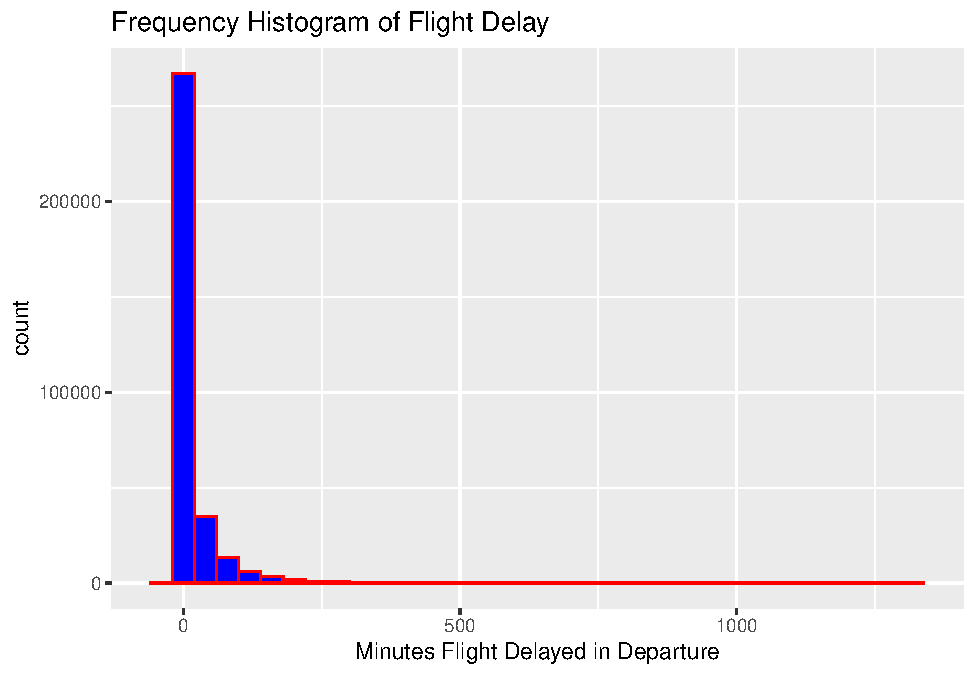
\includegraphics{A3_files/figure-latex/unnamed-chunk-5-1.pdf}

\begin{Shaded}
\begin{Highlighting}[]
\CommentTok{\#As the plot shows, the ratio of the sample standard deviations appear to follow a Normal distribution.}
\end{Highlighting}
\end{Shaded}

\textbf{Q2. c}

\begin{Shaded}
\begin{Highlighting}[]
\FunctionTok{qdata}\NormalTok{(}\SpecialCharTok{\textasciitilde{}}\NormalTok{ ratiosd, }\FunctionTok{c}\NormalTok{(}\FloatTok{0.025}\NormalTok{, }\FloatTok{0.975}\NormalTok{), }\AttributeTok{data=}\NormalTok{boot.ratiosd) }
\end{Highlighting}
\end{Shaded}

\begin{verbatim}
##      2.5%     97.5% 
## 0.8068345 1.0817356
\end{verbatim}

From my result, the 95\% Bootstrap Confidence Interval is
\(0.8008792 \leq \frac{\sigma_{Smoke}}{\sigma_{NonSmoke}} \leq 1.0858073\)

\textbf{Q2. d} the ratio of the sample standard deviations of Weight has
a 95\% of confidents falls in between 0.8008792 and 1.0858073, it shows
\(\sigma_{Smoke}\) is less than \sigma\_\{NonSmoke\}. The Weight of Non
smoke mom's baby has a more clustered distribution around the mean. The
Weight of Smoker mom's baby's has a more spread out distribution around
the mean.

\textbf{Q3 .a}

If mercury levels in walleye fish harvested from the Athabaska River
(downstream of Whitecourt) exceed Heath Canada's action level, then on
average, \(mu_{m} > 1\). If not, on average, \(\mu{m} \leq 1\). The
following are statistical hypotheses:

\[
\begin{eqnarray}
{\rm H}_{0}: \mu_{m} & \leq  (= ) & 1 \hspace{0.2in} \text{(the mean of mercury levels from sampling walleyes did not exceed Heath Canada’s action level)} \\
{\rm H}_{a}: \mu_{m} & > &  1 \hspace{0.2in} \text{(the mean of mercury levels from sampling walleyes exceed Heath Canada’s action level)} \\
\end{eqnarray}
\]

\textbf{Q3. b.} In the context of my statistical hypotheses in part a,
The Type I Error should be that, when the mean mercury (in ppm) of
walleye found downstream from Whitecourt did not exceed Heath Canada's
action level, we make a decision to conclude that the mean mercury
exceed. In a other word, When the null hypothesis is True, Reject the
null hypothesis. The Type II Error should be that, when the mean of
mercury levels from sampling walleyes exceed Heath Canada's action
level, I make a decision to conclude that the mean mercury did not
exceed. In a other word, When the null hypothesis is False, Fail to
Reject the null hypothesis.

\textbf{Q3 c}

\begin{Shaded}
\begin{Highlighting}[]
\NormalTok{mercury.data }\OtherTok{=} \FunctionTok{data.frame}\NormalTok{(}\AttributeTok{mercury =} \FunctionTok{c}\NormalTok{(}\FloatTok{1.2}\NormalTok{,}\FloatTok{1.1}\NormalTok{,}\FloatTok{1.0}\NormalTok{,}\FloatTok{1.0}\NormalTok{,}\FloatTok{1.1}\NormalTok{,}\FloatTok{1.0}\NormalTok{,}\FloatTok{1.0}\NormalTok{,}\FloatTok{1.0}\NormalTok{,}\FloatTok{0.9}\NormalTok{,}\FloatTok{1.1}\NormalTok{,}\FloatTok{1.1}\NormalTok{,}\FloatTok{1.2}\NormalTok{,}\FloatTok{1.0}\NormalTok{,}\FloatTok{1.1}\NormalTok{,}\FloatTok{1.0}\NormalTok{, }\FloatTok{1.1}\NormalTok{,}\FloatTok{1.0}\NormalTok{,}\FloatTok{0.9}\NormalTok{,}\FloatTok{1.0}\NormalTok{,}\FloatTok{1.0}\NormalTok{,}\FloatTok{1.1}\NormalTok{,}\FloatTok{1.0}\NormalTok{,}\FloatTok{1.0}\NormalTok{,}\FloatTok{1.1}\NormalTok{,}\FloatTok{1.2}\NormalTok{,}\FloatTok{1.0}\NormalTok{,}\FloatTok{1.1}\NormalTok{,}\FloatTok{1.0}\NormalTok{,}\FloatTok{1.0}\NormalTok{,}\FloatTok{1.2}\NormalTok{,}\FloatTok{1.1}\NormalTok{))}
\FunctionTok{favstats}\NormalTok{(}\SpecialCharTok{\textasciitilde{}}\NormalTok{mercury, }\AttributeTok{data=}\NormalTok{mercury.data) }\CommentTok{\#will compute various minutes arrive late statistics "conditional" upon airline name}
\end{Highlighting}
\end{Shaded}

\begin{verbatim}
##  min Q1 median  Q3 max     mean         sd  n missing
##  0.9  1      1 1.1 1.2 1.051613 0.08112118 31       0
\end{verbatim}

\begin{Shaded}
\begin{Highlighting}[]
\FunctionTok{head}\NormalTok{(mercury.data)}
\end{Highlighting}
\end{Shaded}

\begin{verbatim}
##   mercury
## 1     1.2
## 2     1.1
## 3     1.0
## 4     1.0
## 5     1.1
## 6     1.0
\end{verbatim}

\begin{Shaded}
\begin{Highlighting}[]
\FunctionTok{ggplot}\NormalTok{(}\AttributeTok{data=}\NormalTok{mercury.data, }\FunctionTok{aes}\NormalTok{(}\AttributeTok{x =} \StringTok{""}\NormalTok{, }\AttributeTok{y =}\NormalTok{ mercury)) }\SpecialCharTok{+} \FunctionTok{geom\_violin}\NormalTok{(}\AttributeTok{col=}\StringTok{"red"}\NormalTok{, }\AttributeTok{fill=}\StringTok{"blue"}\NormalTok{) }\SpecialCharTok{+} \FunctionTok{geom\_boxplot}\NormalTok{(}\AttributeTok{width=}\FloatTok{0.15}\NormalTok{, }\AttributeTok{fill=}\StringTok{"orange"}\NormalTok{, }\AttributeTok{na.rm=}\ConstantTok{TRUE}\NormalTok{) }\SpecialCharTok{+} \FunctionTok{xlab}\NormalTok{(}\StringTok{""}\NormalTok{) }\SpecialCharTok{+} \FunctionTok{ylab}\NormalTok{(}\StringTok{"Departure Delay in Minutes"}\NormalTok{) }\SpecialCharTok{+} \FunctionTok{scale\_x\_discrete}\NormalTok{(}\AttributeTok{breaks=}\ConstantTok{NULL}\NormalTok{) }\SpecialCharTok{+} \FunctionTok{coord\_flip}\NormalTok{() }\SpecialCharTok{+} \FunctionTok{ggtitle}\NormalTok{(}\StringTok{"Violin and Boxplot of the sample of n = 31 mercury (in ppm) from each walleyes from a recent commercial fishing catch downstream from Whitecourt"}\NormalTok{)}
\end{Highlighting}
\end{Shaded}

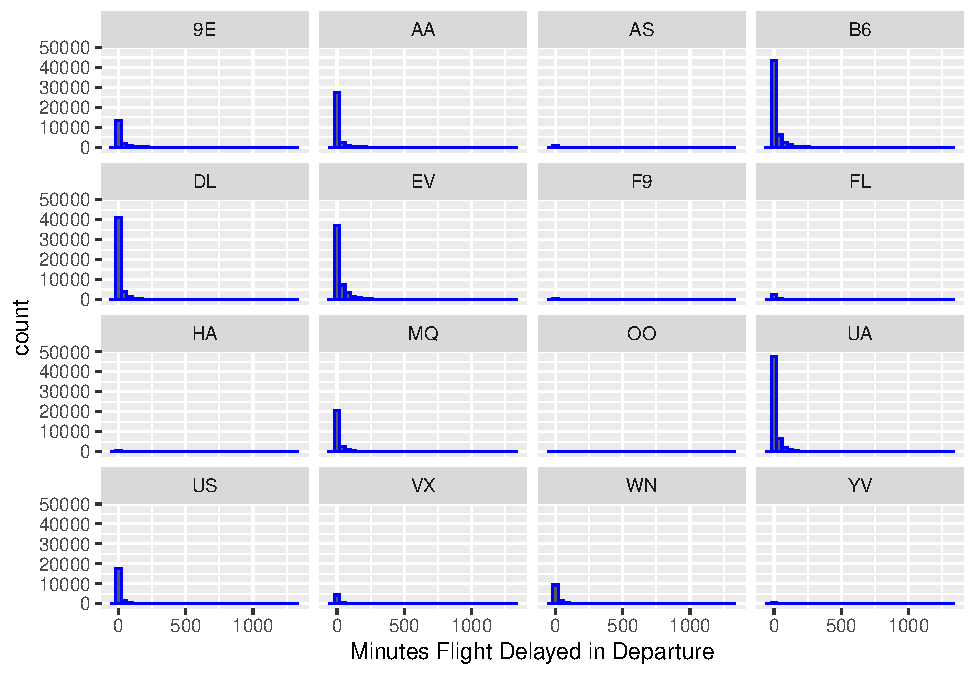
\includegraphics{A3_files/figure-latex/unnamed-chunk-7-1.pdf}

\textbf{Q3 d.} These data does suggest that Health Canada should place a
moritorium on commercial walleye fishing on the Athabaska River
downstream of Whitecourt.

\begin{Shaded}
\begin{Highlighting}[]
\CommentTok{\#I set up The Alpha = 0.05}
\FunctionTok{t.test}\NormalTok{(}\SpecialCharTok{\textasciitilde{}}\NormalTok{ mercury, }\AttributeTok{mu=}\DecValTok{1}\NormalTok{, }\AttributeTok{alternative=}\StringTok{"greater"}\NormalTok{, }\AttributeTok{data=}\NormalTok{mercury.data)}
\end{Highlighting}
\end{Shaded}

\begin{verbatim}
## 
##  One Sample t-test
## 
## data:  mercury
## t = 3.5425, df = 30, p-value = 0.0006595
## alternative hypothesis: true mean is greater than 1
## 95 percent confidence interval:
##  1.026884      Inf
## sample estimates:
## mean of x 
##  1.051613
\end{verbatim}

\begin{Shaded}
\begin{Highlighting}[]
\NormalTok{pvalue }\OtherTok{=} \FloatTok{0.0006595} \CommentTok{\# 0.0006595 \textless{} 0.05}
\CommentTok{\#p{-}value \textless{} Alpha }
\CommentTok{\#Therefore, I reject the null hypothesis.}
\FunctionTok{t.test}\NormalTok{(}\SpecialCharTok{\textasciitilde{}}\NormalTok{mercury, }\AttributeTok{data=}\NormalTok{mercury.data)}\SpecialCharTok{$}\NormalTok{conf}
\end{Highlighting}
\end{Shaded}

\begin{verbatim}
## [1] 1.021857 1.081368
## attr(,"conf.level")
## [1] 0.95
\end{verbatim}

\begin{Shaded}
\begin{Highlighting}[]
\CommentTok{\#A 95\% confidence interval for the mean mercury (in ppm) of walleye found downstream from Whitecourt.}
\CommentTok{\#Is [1.021857, 1.081368].}
\CommentTok{\#In the given scenario, the p{-}value means that the area under the t{-}distribution where t \textgreater{} 3.5425.}
\CommentTok{\#measures how far the test statistic from the H\_0.}
\end{Highlighting}
\end{Shaded}

\textbf{Q4 }

\[
\begin{eqnarray}
{\rm H}_{0}: p  & \leq (=) & \:0.60 \hspace{0.25in} {\rm \text{(the proportion of certified coffee growers in Southern Mexico who are either certified or in the process of being certified, is less or equal than 60%)}} \\
{\rm H}_{0}: p & >& \:0.60 \hspace{0.25in} {\rm \text{(the proportion of certified coffee growers in Southern Mexico who are either certified or in the process of being certified, is more than 60%)}} \\
\end{eqnarray}
\]

\begin{Shaded}
\begin{Highlighting}[]
\NormalTok{Xcertified }\OtherTok{=} \DecValTok{475} \SpecialCharTok{+}\DecValTok{75}
\NormalTok{Xcertified}
\end{Highlighting}
\end{Shaded}

\begin{verbatim}
## [1] 550
\end{verbatim}

I set up \(\alpha = 0.05\) \(n_{SMCG} = 845\). From this, the observed
number who indicated that they were relying on an inheritance to achieve
their financial goals is \(X_{Obs} = 550\).

The Distribution of the Statistic \(X_{Obs}\)

\begin{Shaded}
\begin{Highlighting}[]
\FunctionTok{plot}\NormalTok{(}\FunctionTok{seq}\NormalTok{(}\DecValTok{250}\NormalTok{, }\DecValTok{845}\NormalTok{, }\DecValTok{1}\NormalTok{), }\FunctionTok{dbinom}\NormalTok{(}\FunctionTok{seq}\NormalTok{(}\DecValTok{250}\NormalTok{, }\DecValTok{845}\NormalTok{, }\DecValTok{1}\NormalTok{), }\DecValTok{759}\NormalTok{, }\FloatTok{0.60}\NormalTok{), }\AttributeTok{xlab=}\StringTok{"Values of Sample Sum"}\NormalTok{, }\AttributeTok{ylab=}\StringTok{"P(X = X\_\{Obs\})"}\NormalTok{, }\AttributeTok{type=}\StringTok{"h"}\NormalTok{, }\AttributeTok{col=}\StringTok{"blue"}\NormalTok{, }\AttributeTok{main=}\StringTok{"Distribution of the Test Statistic"}\NormalTok{)}
\FunctionTok{abline}\NormalTok{(}\AttributeTok{v =} \DecValTok{550}\NormalTok{, }\AttributeTok{col=}\StringTok{"red"}\NormalTok{)}
\end{Highlighting}
\end{Shaded}

\includegraphics{A3_files/figure-latex/unnamed-chunk-10-1.pdf}

Computation of the \(P\)-value. Under the assumption/condition that the
null hypothesis \({\rm H}_{0}: p = 0.60\) is true, the \(P\)-value is

\begin{Shaded}
\begin{Highlighting}[]
\NormalTok{pvalue.q4 }\OtherTok{\textless{}{-}} \DecValTok{1} \SpecialCharTok{{-}} \FunctionTok{pbinom}\NormalTok{(}\DecValTok{550}\NormalTok{, }\DecValTok{845}\NormalTok{, }\FloatTok{0.6}\NormalTok{) }\CommentTok{\# computes P(X \textless{}= 550) with n = 845 and the incorporated assummed value of p = 0.6}
\NormalTok{pvalue.q4}
\end{Highlighting}
\end{Shaded}

\begin{verbatim}
## [1] 0.001045019
\end{verbatim}

\begin{Shaded}
\begin{Highlighting}[]
\CommentTok{\#Reject H\_0, as 0.001045019 \textless{} 0.05}
\end{Highlighting}
\end{Shaded}

Reject \({\rm H}_{0}\), as \(0.001045019 < 0.05\)

For a regulated value of \(\alpha = 0.05\), the rejection region is

\begin{Shaded}
\begin{Highlighting}[]
\FunctionTok{qbinom}\NormalTok{(}\FloatTok{0.95}\NormalTok{, }\DecValTok{845}\NormalTok{, }\FloatTok{0.6}\NormalTok{)}
\end{Highlighting}
\end{Shaded}

\begin{verbatim}
## [1] 530
\end{verbatim}

As a result, we have distrust in that assumption and the null hypothesis
is rejected. As a result we conclude from these this sample, that
\(p > 0.60\), or that more than 60\% of certified coffee growers in
Southern Mexico who are either certified or in the process of being
certified.

\textbf{Q5}

\begin{Shaded}
\begin{Highlighting}[]
\FunctionTok{prop.test}\NormalTok{(}\FunctionTok{c}\NormalTok{( }\DecValTok{348} \SpecialCharTok{+} \DecValTok{1}\NormalTok{, }\DecValTok{274} \SpecialCharTok{+} \DecValTok{1}\NormalTok{), }\FunctionTok{c}\NormalTok{(}\DecValTok{670}\SpecialCharTok{+} \DecValTok{2}\NormalTok{, }\DecValTok{376} \SpecialCharTok{+} \DecValTok{2}\NormalTok{), }\AttributeTok{correct=}\ConstantTok{FALSE}\NormalTok{)}
\end{Highlighting}
\end{Shaded}

\begin{verbatim}
## 
##  2-sample test for equality of proportions without continuity
##  correction
## 
## data:  c out of c348 + 1 out of 670 + 2274 + 1 out of 376 + 2
## X-squared = 43.479, df = 1, p-value = 4.284e-11
## alternative hypothesis: two.sided
## 95 percent confidence interval:
##  -0.266833 -0.149503
## sample estimates:
##    prop 1    prop 2 
## 0.5193452 0.7275132
\end{verbatim}

From the result, it shows that difference between two population
proportions are negative. \[
-0.266833 \leq p_{hs} - p_{uni} \leq -0.149503
\\p_{hs} < p_{uni}
\] It means that the proportion of persons with at most a high school
education who disagree the science around vaccinations isn't greater
than the similar proportion of persons with at least an undergraduate
university degree The proportion of persons with at most a high school
education who disagree the science around vaccinations is less than the
similar proportion of persons with at least an undergraduate university
degree.

\textbf{Q6. a}

\[
\begin{eqnarray}
{\rm H}_{0}: p & \leq  & 0.45 \hspace{0.2in} \text{(do not run for office)} \\
{\rm H}_{A}: p & > &  0.45 \hspace{0.2in} \text{(run for office)} \\
\end{eqnarray}
\]

\textbf{Q6 b}

The null hypothesis in (a) is rejected if this count X is greater than
or equal to 20. That is, Reject \({\rm H}_{0}\) if \(X≥20\). Compute the
value of \(\alpha\):

\begin{Shaded}
\begin{Highlighting}[]
\CommentTok{\#Given that you have decided that there is enough statistical }
\CommentTok{\#evidence to support the “mimimum of 45\%”{-}claim if out of n=50 randomly }
\CommentTok{\#chosen voters, at least 20 indicate they will vote for }
\CommentTok{\#this candidate if they run.}
\CommentTok{\#Therefore, The X is set to be 20.}

\CommentTok{\#qbinom(0.95, 50, 0.45)}
\CommentTok{\#1 {-} pbinom(28, 50, 0.45)}
\NormalTok{alpha6 }\OtherTok{=} \FunctionTok{sum}\NormalTok{(}\FunctionTok{dbinom}\NormalTok{(}\DecValTok{20}\SpecialCharTok{:}\DecValTok{50}\NormalTok{, }\DecValTok{50}\NormalTok{, }\FloatTok{0.45}\NormalTok{))}
\NormalTok{alpha6}
\end{Highlighting}
\end{Shaded}

\begin{verbatim}
## [1] 0.8026321
\end{verbatim}

\textbf{Q6. c}

\begin{Shaded}
\begin{Highlighting}[]
\CommentTok{\#I think the creator of the question wants us to compute the Type II Error here.}

\CommentTok{\#It is the Type II Error if and only if the statistical hypotheses set to be}
\CommentTok{\#H\_0 is P \textgreater{}= 0.45, H\_a is p \textless{} 0.45.}

\CommentTok{\#However, I set up my statistical hypotheses as H\_0: p\textless{}= 0.45, H\_a: p \textgreater{}0.45}
\CommentTok{\#This makes the part c becomes that, when H\_0 is Ture, Reject H\_0, }
\CommentTok{\#which is a Type I Error. }

\CommentTok{\#From what I learn in the lecture, There is no wrong setting up for }
\CommentTok{\#the statistical hypotheses as long as the following steps can make sense.}
\CommentTok{\#And I am certain that my H\_0 and H\_a can carry out the Hypothesis Testing}
\CommentTok{\#with no problem.}

\CommentTok{\#Therefore, it is not my fault that part c, d and e makes less sense under }
\CommentTok{\#the statistical hypotheses I came up with.}

\NormalTok{probc }\OtherTok{=} \FunctionTok{sum}\NormalTok{(}\FunctionTok{dbinom}\NormalTok{(}\DecValTok{20}\SpecialCharTok{:}\DecValTok{50}\NormalTok{, }\DecValTok{50}\NormalTok{, }\FloatTok{0.42}\NormalTok{))}
\NormalTok{probc }
\end{Highlighting}
\end{Shaded}

\begin{verbatim}
## [1] 0.663807
\end{verbatim}

\begin{Shaded}
\begin{Highlighting}[]
\CommentTok{\#1 {-} pbinom(19, 50, 0.42)}
\CommentTok{\#The probability that you will conclude they should run for office,}
\CommentTok{\#if the candidate were to receive 42\% of the vote.}

\CommentTok{\#This is the probability that If H\_0 is true, Reject H\_0.}
\CommentTok{\#(in this case, H\_0:p \textless{}= 0.45)}
\end{Highlighting}
\end{Shaded}

\textbf{Q6. d}

\begin{Shaded}
\begin{Highlighting}[]
\CommentTok{\#Refer to my thought in part c, }
\CommentTok{\#those are probabilities of H\_0 is true,Reject H\_0, }
\CommentTok{\#with different values of p \textless{}= 0.45}
\NormalTok{proportionofvote }\OtherTok{=} \FunctionTok{c}\NormalTok{(}\FloatTok{0.41}\NormalTok{,}\FloatTok{0.40}\NormalTok{,}\FloatTok{0.39}\NormalTok{,}\FloatTok{0.38}\NormalTok{,}\FloatTok{0.35}\NormalTok{, }\FloatTok{0.30}\NormalTok{)}


\NormalTok{proboutcomes }\OtherTok{=} \DecValTok{1} \SpecialCharTok{{-}} \FunctionTok{pbinom}\NormalTok{(}\DecValTok{19}\NormalTok{,}\DecValTok{50}\NormalTok{,proportionofvote)}

\NormalTok{df.proboutcomes }\OtherTok{\textless{}{-}} \FunctionTok{data.frame}\NormalTok{(proportionofvote,proboutcomes)}
\FunctionTok{head}\NormalTok{(df.proboutcomes)}
\end{Highlighting}
\end{Shaded}

\begin{verbatim}
##   proportionofvote proboutcomes
## 1             0.41    0.6099048
## 2             0.40    0.5535236
## 3             0.39    0.4957191
## 4             0.38    0.4376490
## 5             0.35    0.2735637
## 6             0.30    0.0848026
\end{verbatim}

\begin{Shaded}
\begin{Highlighting}[]
\FunctionTok{ggplot}\NormalTok{(}\AttributeTok{data=}\NormalTok{df.proboutcomes, }\FunctionTok{aes}\NormalTok{(}\AttributeTok{x =}\NormalTok{ proportionofvote, }\AttributeTok{y =}\NormalTok{ proboutcomes)) }\SpecialCharTok{+} \FunctionTok{geom\_point}\NormalTok{(}\AttributeTok{fill=}\StringTok{"blue"}\NormalTok{) }\SpecialCharTok{+} \FunctionTok{xlab}\NormalTok{(}\StringTok{"Values of p (Proportion of Reveiving Votes) "}\NormalTok{) }\SpecialCharTok{+} \FunctionTok{ylab}\NormalTok{(}\StringTok{"Probabiltiy of Reject H\_0"}\NormalTok{)}
\end{Highlighting}
\end{Shaded}

\includegraphics{A3_files/figure-latex/unnamed-chunk-16-1.pdf}

\textbf{Q6. e}

\begin{Shaded}
\begin{Highlighting}[]
\CommentTok{\#The graph in part (d) tells that the probability that }
\CommentTok{\#I will conclude they should run for office }
\CommentTok{\#is proportional to the value of p which are the proportion of vote received.}
\CommentTok{\#In another word, as the the the candidate receives more votes,}
\CommentTok{\#the probability of concluding that he should run for the office is increasing. }


\CommentTok{\#As those are Type I Errors with different values of p \textless{}= 0.45, }
\CommentTok{\#It means that the chance of making a Type I Error is very high, }
\CommentTok{\#when the p value is approaching to the upper bound of H\_0, where p = 0.45.}
\CommentTok{\#In another word, The probability of Type I Error appearing is too high.}

\CommentTok{\#The statistical test can be improved by changing the rejection region.}
\CommentTok{\#For a regulated value of alpha = 0.05, the rejection region is x \textgreater{} 28}
\CommentTok{\#And the value of alpha should be change to 0.04437937}
\CommentTok{\#It insures that the statistical hypotheses is more accurate.}
\FunctionTok{qbinom}\NormalTok{(}\FloatTok{0.95}\NormalTok{, }\DecValTok{50}\NormalTok{, }\FloatTok{0.45}\NormalTok{)}
\end{Highlighting}
\end{Shaded}

\begin{verbatim}
## [1] 28
\end{verbatim}

\begin{Shaded}
\begin{Highlighting}[]
\NormalTok{alphae }\OtherTok{=} \DecValTok{1} \SpecialCharTok{{-}} \FunctionTok{pbinom}\NormalTok{(}\DecValTok{28}\NormalTok{, }\DecValTok{50}\NormalTok{, }\FloatTok{0.45}\NormalTok{)}
\NormalTok{alphae}
\end{Highlighting}
\end{Shaded}

\begin{verbatim}
## [1] 0.04437937
\end{verbatim}

\[
\text{Reject the null hypothesis if} \:\: \{X_{Obs}: X > 28\}
\]

\textbf{Q7. a}

\begin{Shaded}
\begin{Highlighting}[]
\NormalTok{df.q7 }\OtherTok{=} \FunctionTok{read.csv}\NormalTok{(}\StringTok{"http://people.ucalgary.ca/\textasciitilde{}jbstall/DataFiles/bookprices.csv"}\NormalTok{)}
\CommentTok{\#head(df.q7)}
\NormalTok{df.q7 }\OtherTok{=}\NormalTok{ df.q7 }\SpecialCharTok{\%\textgreater{}\%}
  \FunctionTok{mutate}\NormalTok{(}\AttributeTok{Diff =}\NormalTok{ UsedBkStore }\SpecialCharTok{{-}}\NormalTok{ UsedAmazon) }\CommentTok{\#create a new variable called Diff = price of camera at JR {-} price of same camera at BH}
\FunctionTok{head}\NormalTok{(df.q7)}
\end{Highlighting}
\end{Shaded}

\begin{verbatim}
##   UsedBkStore UsedAmazon   Diff
## 1      160.46     128.95  31.51
## 2       82.05      34.40  47.65
## 3       96.08      30.41  65.67
## 4       96.71     110.99 -14.28
## 5       77.96      33.99  43.97
## 6      104.96      20.00  84.96
\end{verbatim}

Given that these data were collected using a \textbf{Matched Pairs
Experimental Design}, the difference is defined as

\[
d_{i} = x_{UsedBkStore, i} - x_{UsedAmazon, i}
\]

the statistical hypothesis to be tested is

\[
\begin{eqnarray}
{\rm H}_{0}: \mu_{d} & \leq  (= ) & 0 \hspace{0.2in} \text{(the mean of a population of differences is at most equal to zero)} \\
{\rm H}_{A}: \mu_{d} & > &  0 \hspace{0.2in} \text{(the mean of a population of differences is more than zero)} \\
\end{eqnarray}
\]

I set up the \(\alpha = 0.05\)

\begin{Shaded}
\begin{Highlighting}[]
\CommentTok{\#Find p{-}value by using t.test}
\FunctionTok{t.test}\NormalTok{(}\SpecialCharTok{\textasciitilde{}}\NormalTok{Diff, }\AttributeTok{mu=}\DecValTok{0}\NormalTok{, }\AttributeTok{alternative=}\StringTok{"two.sided"}\NormalTok{, }\AttributeTok{data=}\NormalTok{df.q7)}
\end{Highlighting}
\end{Shaded}

\begin{verbatim}
## 
##  One Sample t-test
## 
## data:  Diff
## t = 3.0357, df = 14, p-value = 0.008898
## alternative hypothesis: true mean is not equal to 0
## 95 percent confidence interval:
##   7.474595 43.461405
## sample estimates:
## mean of x 
##    25.468
\end{verbatim}

\begin{Shaded}
\begin{Highlighting}[]
\CommentTok{\#p{-}value is 0.008898}
\end{Highlighting}
\end{Shaded}

Because \(p-value < \alpha\), I Reject \(H_{0}: \mu_{d} \leq(=) 0\). I
conclude that the price of a used textbook at the University of Calgary
Bookstore is more when compared to the price of a used text book on
Amazon.ca.

\textbf{Q7. b} The inferences made about the mean different in the price
of used textbooks between University of Calgary Bookstore and Amazon.ca
are made upon the condition that the differences follow a Normal
distribution/can be modeled by the Normal probability model.

\begin{Shaded}
\begin{Highlighting}[]
\FunctionTok{ggplot}\NormalTok{(}\AttributeTok{data=}\NormalTok{df.q7, }\FunctionTok{aes}\NormalTok{(}\AttributeTok{sample =}\NormalTok{ Diff)) }\SpecialCharTok{+} \FunctionTok{stat\_qq}\NormalTok{(}\AttributeTok{size=}\DecValTok{2}\NormalTok{, }\AttributeTok{col=}\StringTok{\textquotesingle{}blue\textquotesingle{}}\NormalTok{) }\SpecialCharTok{+} \FunctionTok{stat\_qq\_line}\NormalTok{(}\AttributeTok{col=}\StringTok{\textquotesingle{}red\textquotesingle{}}\NormalTok{) }\SpecialCharTok{+} \FunctionTok{ggtitle}\NormalTok{(}\StringTok{"Normal Probability Plot of Difference: UsedBkStore {-} UsedAmazon"}\NormalTok{)}
\end{Highlighting}
\end{Shaded}

\includegraphics{A3_files/figure-latex/unnamed-chunk-20-1.pdf}

\begin{Shaded}
\begin{Highlighting}[]
\CommentTok{\#As the plot shows this condition is satisfied.}
\end{Highlighting}
\end{Shaded}

\textbf{Q8} the statistical hypothesis to be tested is \[
\begin{eqnarray}
{\rm H}_{0}: p_{psd}  & = & \:0.62 \hspace{0.25in} {\rm \text{(the proportion of residents of a certain municipality is the same as the provincial proportion)}} \\
{\rm H}_{0}: p_{psd} & \neq & \:0.62 \hspace{0.25in} {\rm \text{(the proportion of residents of a certain municipality differs from the provincial proportion)}} \\
\end{eqnarray}
\] I set up the \(\alpha = 0.05\)

Obtain a test statistic, a smaple of 250 randomly chosen adults yielded
145 completed some form of post-secondary education. X = 145 which is
the test statistic. \(n = 250\), \(X_{Obs} = 145\)

\begin{Shaded}
\begin{Highlighting}[]
\CommentTok{\#Calculate the p{-}value}
\FunctionTok{binom.test}\NormalTok{(}\DecValTok{145}\NormalTok{, }\DecValTok{250}\NormalTok{, }\FloatTok{0.62}\NormalTok{, }\AttributeTok{ci.method=}\StringTok{"plus4"}\NormalTok{)}
\end{Highlighting}
\end{Shaded}

\begin{verbatim}
## 
##  Exact binomial test (Plus 4 CI)
## 
## data:  145 out of 250
## number of successes = 145, number of trials = 250, p-value = 0.1932
## alternative hypothesis: true probability of success is not equal to 0.62
## 95 percent confidence interval:
##  0.5180179 0.6394624
## sample estimates:
## probability of success 
##                   0.58
\end{verbatim}

The 95\% Confidence Interval for \(p_{psd}\) is: \[
0.5180179  \leq p_{psd} \leq 0.6394624
\] Where the \(H_{0}\) falls in this Confidence Interval.

The \(p_value = 0.1932\), \(p_value >\alpha\). I Fail to Reject
\(H_{0}\).

Thus, I conclude that the proportion of residents of a certain
municipality is the same as the provincial proportion.

In the context of these data, the p-value is the probability that
another sample of n=250 randomly chosen adults aged 25 - 64 living in
this municipality will yield more condemning evidence than the test
statistic we have this time which is 145, assuming that the null
hypothesis \(p = 0.62\) is correct. Where the null hypothesis is the
proportion of residents of a certain municipality is the same as the
provincial proportion.

For a two tail test, p - value is the area under the binomial
probability distribution curve values that far from the absolutely
values of test statistic and the negative absolutely values of test
statistic in both directions. Each area represents half of the p-value.

\textbf{Q9 a }

\begin{Shaded}
\begin{Highlighting}[]
\NormalTok{n1 }\OtherTok{=} \DecValTok{1000}
\NormalTok{x1 }\OtherTok{=} \DecValTok{561}
\NormalTok{n2 }\OtherTok{=} \DecValTok{1010}
\NormalTok{x2 }\OtherTok{=} \DecValTok{601}
\FunctionTok{prop.test}\NormalTok{(}\FunctionTok{c}\NormalTok{(x1 }\SpecialCharTok{+} \DecValTok{1}\NormalTok{, x2 }\SpecialCharTok{+} \DecValTok{1}\NormalTok{), }\FunctionTok{c}\NormalTok{(n1 }\SpecialCharTok{+} \DecValTok{2}\NormalTok{, n2 }\SpecialCharTok{+} \DecValTok{2}\NormalTok{), }\AttributeTok{conf.level=}\FloatTok{0.95}\NormalTok{, }\AttributeTok{correct=}\ConstantTok{FALSE}\NormalTok{)}\SpecialCharTok{$}\NormalTok{conf }
\end{Highlighting}
\end{Shaded}

\begin{verbatim}
## [1] -0.077100209  0.009133376
## attr(,"conf.level")
## [1] 0.95
\end{verbatim}

The 95\% Confidence Interval for \(p_{2019} - p_{2012}\) is: \[
-0.077100209    \leq p_{2019} - p_{2012} \leq 0.009133376
\]

\textbf{Q9 b } The result in part (a) shows that there is no
statistically significant difference between \(p_{2019}\) and
\(p_{2012}\). Because the difference between the proportion of Canadians
who currently support a ban on single-use plastics and the proportion of
Canadians who supported such a ban in 2012 falls in the interval
{[}-0.077100209, 0.009133376{]}. Between a negative value and a positive
value, it could happen if \(p_{2019} - p_{2012} = 0\).

\textbf{Q10 a} The statistical hypothesis to be tested is \[
\begin{eqnarray}
{\rm H}_{0}: \mu_{w}  & = & \:500 \hspace{0.25in} {\rm \text{(the mean weight of cereals is 500 grams)}} \\
{\rm H}_{a}: \mu_{w} & < & \:500 \hspace{0.25in} {\rm \text{(the mean weight of cereals is less than 500 grams)}} \\
\end{eqnarray}
\] I set up the \(\alpha = 0.05\)

\begin{Shaded}
\begin{Highlighting}[]
\NormalTok{cereal.data }\OtherTok{=} \FunctionTok{data.frame}\NormalTok{(}\AttributeTok{gram =} \FunctionTok{c}\NormalTok{(}\FloatTok{497.2}\NormalTok{,}\FloatTok{499.9}\NormalTok{,}\FloatTok{495.8}\NormalTok{,}\FloatTok{514.2}\NormalTok{,}\FloatTok{490.0}\NormalTok{,}\FloatTok{498.3}\NormalTok{,}\FloatTok{495.1}\NormalTok{,}\FloatTok{486.7}\NormalTok{))}
\FunctionTok{head}\NormalTok{(cereal.data)}
\end{Highlighting}
\end{Shaded}

\begin{verbatim}
##    gram
## 1 497.2
## 2 499.9
## 3 495.8
## 4 514.2
## 5 490.0
## 6 498.3
\end{verbatim}

\begin{Shaded}
\begin{Highlighting}[]
\FunctionTok{favstats}\NormalTok{(}\SpecialCharTok{\textasciitilde{}}\NormalTok{gram, }\AttributeTok{data =}\NormalTok{ cereal.data)}
\end{Highlighting}
\end{Shaded}

\begin{verbatim}
##    min      Q1 median    Q3   max   mean       sd n missing
##  486.7 493.825  496.5 498.7 514.2 497.15 8.158606 8       0
\end{verbatim}

\begin{Shaded}
\begin{Highlighting}[]
\FunctionTok{ggplot}\NormalTok{(}\AttributeTok{data=}\NormalTok{cereal.data, }\FunctionTok{aes}\NormalTok{(}\AttributeTok{sample =}\NormalTok{ gram)) }\SpecialCharTok{+} \FunctionTok{stat\_qq}\NormalTok{(}\AttributeTok{size=}\DecValTok{2}\NormalTok{, }\AttributeTok{col=}\StringTok{"blue"}\NormalTok{) }\SpecialCharTok{+} \FunctionTok{stat\_qqline}\NormalTok{(}\AttributeTok{col=}\StringTok{"red"}\NormalTok{) }\SpecialCharTok{+} \FunctionTok{ggtitle}\NormalTok{(}\StringTok{"Normal Probability Plot n = 8 Weights the contents of each Box Cereal from Different Stores"}\NormalTok{)}
\end{Highlighting}
\end{Shaded}

\includegraphics{A3_files/figure-latex/unnamed-chunk-23-1.pdf}

\begin{Shaded}
\begin{Highlighting}[]
\CommentTok{\#n = 8}
\CommentTok{\#Inspected a Normal Probability plot of these data, it appeared to be Normal (for the most part).}
\end{Highlighting}
\end{Shaded}

\begin{Shaded}
\begin{Highlighting}[]
\NormalTok{mu}\FloatTok{.0} \OtherTok{\textless{}{-}} \DecValTok{500}
\NormalTok{dof }\OtherTok{\textless{}{-}} \FunctionTok{favstats}\NormalTok{(}\SpecialCharTok{\textasciitilde{}}\NormalTok{gram, }\AttributeTok{data =}\NormalTok{ cereal.data)}\SpecialCharTok{$}\NormalTok{n }\SpecialCharTok{{-}} \DecValTok{1} \CommentTok{\#set the degrees of freedom to n {-} 1}
\NormalTok{t.obs }\OtherTok{\textless{}{-}}\NormalTok{ (}\FunctionTok{favstats}\NormalTok{(}\SpecialCharTok{\textasciitilde{}}\NormalTok{gram, }\AttributeTok{data =}\NormalTok{ cereal.data)}\SpecialCharTok{$}\NormalTok{mean }\SpecialCharTok{{-}}\NormalTok{ mu}\FloatTok{.0}\NormalTok{)}\SpecialCharTok{/}\NormalTok{(}\FunctionTok{favstats}\NormalTok{(}\SpecialCharTok{\textasciitilde{}}\NormalTok{gram, }\AttributeTok{data =}\NormalTok{ cereal.data)}\SpecialCharTok{$}\NormalTok{sd }\SpecialCharTok{/}\FunctionTok{sqrt}\NormalTok{(}\FunctionTok{favstats}\NormalTok{(}\SpecialCharTok{\textasciitilde{}}\NormalTok{gram, }\AttributeTok{data =}\NormalTok{ cereal.data)}\SpecialCharTok{$}\NormalTok{n))}
\NormalTok{t.obs}
\end{Highlighting}
\end{Shaded}

\begin{verbatim}
## [1] -0.9880385
\end{verbatim}

\begin{Shaded}
\begin{Highlighting}[]
\FunctionTok{pt}\NormalTok{(t.obs, }\DecValTok{7}\NormalTok{)}
\end{Highlighting}
\end{Shaded}

\begin{verbatim}
## [1] 0.1780239
\end{verbatim}

\begin{Shaded}
\begin{Highlighting}[]
\FunctionTok{t.test}\NormalTok{(}\SpecialCharTok{\textasciitilde{}}\NormalTok{ gram, }\AttributeTok{mu=}\DecValTok{500}\NormalTok{, }\AttributeTok{alternative=} \StringTok{"less"}\NormalTok{, }\AttributeTok{data=}\NormalTok{cereal.data) }\CommentTok{\#sets mu = 500 (H0 is true) and indicates sign in Ha}
\end{Highlighting}
\end{Shaded}

\begin{verbatim}
## 
##  One Sample t-test
## 
## data:  gram
## t = -0.98804, df = 7, p-value = 0.178
## alternative hypothesis: true mean is less than 500
## 95 percent confidence interval:
##      -Inf 502.6149
## sample estimates:
## mean of x 
##    497.15
\end{verbatim}

\(T_{Obs} = 0.1604\) \[
P-\text{value} = 0.178
\] Because \(P-\text{value} > \alpha\), I Fail to Reject
\({\rm H}_{0}\). Thus, I conclude that the mean of Cereals is 500 grams.
Usman is getting the amount of cereal as stated on the box.

\textbf{Q10 b}

\begin{Shaded}
\begin{Highlighting}[]
\NormalTok{ntimes }\OtherTok{=} \DecValTok{1000}  
\NormalTok{nsize }\OtherTok{=} \DecValTok{8}     
\NormalTok{Tboot }\OtherTok{=} \FunctionTok{numeric}\NormalTok{(ntimes)  }
\NormalTok{mu}\FloatTok{.0} \OtherTok{=} \FunctionTok{favstats}\NormalTok{(}\SpecialCharTok{\textasciitilde{}}\NormalTok{gram, }\AttributeTok{data =}\NormalTok{ cereal.data)}\SpecialCharTok{$}\NormalTok{mean}
\NormalTok{dof }\OtherTok{=}\NormalTok{ nsize }\SpecialCharTok{{-}} \DecValTok{1}
\NormalTok{origdata }\OtherTok{=} \FunctionTok{c}\NormalTok{(}\FloatTok{497.2}\NormalTok{,}\FloatTok{499.9}\NormalTok{,}\FloatTok{495.8}\NormalTok{,}\FloatTok{514.2}\NormalTok{,}\FloatTok{490.0}\NormalTok{,}\FloatTok{498.3}\NormalTok{,}\FloatTok{495.1}\NormalTok{,}\FloatTok{486.7}\NormalTok{)}
\ControlFlowTok{for}\NormalTok{(i }\ControlFlowTok{in} \DecValTok{1}\SpecialCharTok{:}\NormalTok{ntimes) }\CommentTok{\#start the for loop, run 1000 times}
\NormalTok{\{   databoot }\OtherTok{=} \FunctionTok{sample}\NormalTok{(origdata, nsize, }\AttributeTok{replace=}\ConstantTok{TRUE}\NormalTok{)  }\CommentTok{\#data of nsize, sampling w replacement}
\NormalTok{    Tboot[i] }\OtherTok{=}\NormalTok{  (}\FunctionTok{favstats}\NormalTok{(databoot)}\SpecialCharTok{$}\NormalTok{mean }\SpecialCharTok{{-}}\NormalTok{ mu}\FloatTok{.0}\NormalTok{)}\SpecialCharTok{/}\NormalTok{(}\FunctionTok{favstats}\NormalTok{(databoot)}\SpecialCharTok{$}\NormalTok{sd }\SpecialCharTok{/}\FunctionTok{sqrt}\NormalTok{(}\FunctionTok{favstats}\NormalTok{(databoot)}\SpecialCharTok{$}\NormalTok{n))}
\NormalTok{\} }\CommentTok{\#close the for loop}
\NormalTok{Tbootstrap }\OtherTok{=} \FunctionTok{data.frame}\NormalTok{(Tboot)}
\FunctionTok{head}\NormalTok{(Tbootstrap)}
\end{Highlighting}
\end{Shaded}

\begin{verbatim}
##         Tboot
## 1 -0.34233043
## 2  1.37984220
## 3 -2.36899576
## 4 -1.82916887
## 5 -0.04108092
## 6 -0.61097094
\end{verbatim}

\begin{Shaded}
\begin{Highlighting}[]
\FunctionTok{ggplot}\NormalTok{(}\AttributeTok{data=}\NormalTok{Tbootstrap, }\FunctionTok{aes}\NormalTok{(}\AttributeTok{x =}\NormalTok{ Tboot)) }\SpecialCharTok{+} \FunctionTok{geom\_histogram}\NormalTok{(}\AttributeTok{col=}\StringTok{\textquotesingle{}blue\textquotesingle{}}\NormalTok{, }\AttributeTok{fill=}\StringTok{\textquotesingle{}yellow\textquotesingle{}}\NormalTok{, }\AttributeTok{binwidth=}\FloatTok{0.5}\NormalTok{) }\SpecialCharTok{+} \FunctionTok{ylab}\NormalTok{(}\StringTok{"Count"}\NormalTok{) }\SpecialCharTok{+} \FunctionTok{ggtitle}\NormalTok{(}\StringTok{"Distribution of Bootstrap Statisic:  t{-}distriubution"}\NormalTok{) }\SpecialCharTok{+} \FunctionTok{geom\_vline}\NormalTok{(}\AttributeTok{xintercept =} \SpecialCharTok{{-}}\FloatTok{0.9880385}\NormalTok{, }\AttributeTok{col=}\StringTok{"black"}\NormalTok{)}
\end{Highlighting}
\end{Shaded}

\includegraphics{A3_files/figure-latex/unnamed-chunk-26-1.pdf}

\begin{Shaded}
\begin{Highlighting}[]
\FunctionTok{qdata}\NormalTok{(}\SpecialCharTok{\textasciitilde{}}\NormalTok{ Tboot, }\FloatTok{0.05}\NormalTok{ , }\AttributeTok{data=}\NormalTok{Tbootstrap)}
\end{Highlighting}
\end{Shaded}

\begin{verbatim}
##        5% 
## -2.386964
\end{verbatim}

\begin{Shaded}
\begin{Highlighting}[]
\CommentTok{\#The  5th percentile of the distribution is {-}2.459316 }
\end{Highlighting}
\end{Shaded}

\textbf{Q10 c}

\begin{Shaded}
\begin{Highlighting}[]
\NormalTok{X\_bar }\OtherTok{=} \FunctionTok{favstats}\NormalTok{(}\SpecialCharTok{\textasciitilde{}}\NormalTok{gram, }\AttributeTok{data =}\NormalTok{ cereal.data)}\SpecialCharTok{$}\NormalTok{mean}
\NormalTok{S }\OtherTok{=} \FunctionTok{favstats}\NormalTok{(}\SpecialCharTok{\textasciitilde{}}\NormalTok{gram, }\AttributeTok{data =}\NormalTok{ cereal.data)}\SpecialCharTok{$}\NormalTok{sd}
\NormalTok{n }\OtherTok{=} \FunctionTok{favstats}\NormalTok{(}\SpecialCharTok{\textasciitilde{}}\NormalTok{gram, }\AttributeTok{data =}\NormalTok{ cereal.data)}\SpecialCharTok{$}\NormalTok{n}
\NormalTok{tboot5th }\OtherTok{=} \FunctionTok{qdata}\NormalTok{(}\SpecialCharTok{\textasciitilde{}}\NormalTok{ Tboot, }\FloatTok{0.05}\NormalTok{ , }\AttributeTok{data=}\NormalTok{Tbootstrap)}
\NormalTok{X\_bar5th }\OtherTok{=}\NormalTok{ X\_bar }\SpecialCharTok{{-}}\NormalTok{ tboot5th }\SpecialCharTok{*}\NormalTok{ (S}\SpecialCharTok{/}\NormalTok{n)}
\NormalTok{X\_bar5th}
\end{Highlighting}
\end{Shaded}

\begin{verbatim}
##       5% 
## 499.5843
\end{verbatim}

\begin{Shaded}
\begin{Highlighting}[]
\CommentTok{\#It is very close to 500}
\CommentTok{\#The result infer the same thing as the result in part (a).}
\CommentTok{\#I Fail to Reject H\_0.}
\CommentTok{\#I conclude that the mean of Cereals is 500 grams.}
\CommentTok{\#Usman is getting the amount of cereal as stated on the box.}
\end{Highlighting}
\end{Shaded}

\textbf{Q11 a} \[
{\rm H}_{0}: \beta   = 2 \hspace{0.5in} {\rm H}_{A}: \beta   < 2
\\
\text{Reject} \:\:{\rm H}_{0}: \{X_{Min} < 2.018\}
\] \[
\begin{eqnarray}
\alpha & = & P(\text{Reject}\:\:{\rm H}_{0} | {\rm H}_{0} \: \text{is true}) \\
       & = & P(X_{Min} < 2.018 | \beta   = 2) \\
       & = & P(2 < X_{Min} < 2.018) \\
\end{eqnarray}
\]

\begin{Shaded}
\begin{Highlighting}[]
\NormalTok{pdfxmin }\OtherTok{=} \ControlFlowTok{function}\NormalTok{(x) \{}
  \DecValTok{6}\SpecialCharTok{*}\FunctionTok{exp}\NormalTok{(}\SpecialCharTok{{-}}\DecValTok{6}\SpecialCharTok{*}\NormalTok{(x}\DecValTok{{-}2}\NormalTok{))}
\NormalTok{\}}
\FunctionTok{integrate}\NormalTok{(pdfxmin, }\AttributeTok{lower =} \DecValTok{2}\NormalTok{, }\AttributeTok{upper =} \FloatTok{2.018}\NormalTok{)}\SpecialCharTok{$}\NormalTok{value}
\end{Highlighting}
\end{Shaded}

\begin{verbatim}
## [1] 0.1023724
\end{verbatim}

The value of \(\alpha\) was used in the derivation of this statistical
test is \(\alpha = 0.1023724\)

\textbf{Q11 b} Assuming \(H_{0}\) is True.

\begin{Shaded}
\begin{Highlighting}[]
\NormalTok{obs }\OtherTok{=} \FunctionTok{c}\NormalTok{(}\FloatTok{2.95}\NormalTok{,}\FloatTok{2.21}\NormalTok{,}\FloatTok{2.43}\NormalTok{,}\FloatTok{2.11}\NormalTok{,}\FloatTok{2.77}\NormalTok{,}\FloatTok{3.12}\NormalTok{)}
\NormalTok{xminobs }\OtherTok{=} \FunctionTok{favstats}\NormalTok{(obs)}\SpecialCharTok{$}\NormalTok{min}
\NormalTok{xminobs}
\end{Highlighting}
\end{Shaded}

\begin{verbatim}
## [1] 2.11
\end{verbatim}

\begin{Shaded}
\begin{Highlighting}[]
\FunctionTok{integrate}\NormalTok{(pdfxmin, }\AttributeTok{lower =} \DecValTok{2}\NormalTok{, }\AttributeTok{upper =}\NormalTok{ xminobs)}\SpecialCharTok{$}\NormalTok{value }\CommentTok{\#Calculating the p{-}value}
\end{Highlighting}
\end{Shaded}

\begin{verbatim}
## [1] 0.4831487
\end{verbatim}

\[
P-\text{value} = 0.1455216 
\] Because \(P-\text{value} > \alpha\), I Fail to Reject
\({\rm H}_{0}\). This sample does support the null hypothesis above.

\textbf{Q11 c} Calculate the Type II Error \[
\begin{eqnarray}
\beta & = & P(\text{Fail to Reject}\:\:{\rm H}_{0} | {\rm H}_{0} \: \text{is false}) \\
       & = & P(X_{Min} \geq 2.018 | \beta    = 1.8) \\
       & = & 1- P(X_{Min} < 2.018 | \beta    = 1.8) \\
\end{eqnarray}
\]

\begin{Shaded}
\begin{Highlighting}[]
\NormalTok{pdfxminc }\OtherTok{=} \ControlFlowTok{function}\NormalTok{(x) \{}
  \DecValTok{6}\SpecialCharTok{*}\FunctionTok{exp}\NormalTok{(}\SpecialCharTok{{-}}\DecValTok{6}\SpecialCharTok{*}\NormalTok{(x}\FloatTok{{-}1.8}\NormalTok{))}
\NormalTok{\}}

\DecValTok{1}\SpecialCharTok{{-}} \FunctionTok{integrate}\NormalTok{(pdfxminc, }\AttributeTok{lower =} \FloatTok{1.8}\NormalTok{, }\AttributeTok{upper =} \FloatTok{2.018}\NormalTok{)}\SpecialCharTok{$}\NormalTok{value}
\end{Highlighting}
\end{Shaded}

\begin{verbatim}
## [1] 0.2703602
\end{verbatim}

\begin{Shaded}
\begin{Highlighting}[]
\CommentTok{\#Or just do}
\CommentTok{\#integrate(pdfxmin, lower = 2.018, upper = Inf)}
\CommentTok{\#Getting same result.}
\end{Highlighting}
\end{Shaded}

\textbf{Q8 d}

\(\alpha = 0.2\)

\[
\begin{eqnarray}
\alpha & = & P(\text{Reject}\:\:{\rm H}_{0} | {\rm H}_{0} \: \text{is true}) \\
0.2       & = & P(X_{Min} < t | \beta    = 2) \\
\end{eqnarray}
\] \[
 \int_{2}^{t} 6e^{-6(x_{Min}-2)} \,dx = 0.2
\] Solve for t. I solved the t by hand with u substitution, the solution
is too complicated to type. \[
 t = \frac{12 - \log(0.8) }{{6}} \approx 2.0372
\]

\begin{Shaded}
\begin{Highlighting}[]
\FunctionTok{integrate}\NormalTok{(pdfxmin, }\AttributeTok{lower =} \DecValTok{2}\NormalTok{, }\AttributeTok{upper =} \FloatTok{2.0372}\NormalTok{)}\SpecialCharTok{$}\NormalTok{value}
\end{Highlighting}
\end{Shaded}

\begin{verbatim}
## [1] 0.2000452
\end{verbatim}

The value of \(X_{Min}\) is 2.0372

\end{document}
